\chapter{Implementacja}

Tworzenie projektu odbyło się metodyką przyrostowo-ewolucyjną. Metodyka ta pozwala na szybką adaptację i elastyczność, która jest kluczowa w przypadku projektów, które mogą ulegać zmianom w czasie realizacji. Tworzenie systemu odbyło się w dwóch etapach, fazie planowanie i fazie implementacji. Faza planowania dotyczyła określenia celu projektu, funkcjonalności systemu i wypełnienia dokumentacji. Faza implementacji odbywała się w sprintach, które zazwyczaj trwały od 2 do 3 tygodni.

\section{Faza planowania}

Na samym początku przeprowadzona została burza mózgów w celu wymyślenia tematu naszego projektu \cite{osborn1953}. Po analizie potencjalnych tematów zespół zdecydował się na aplikację do uczenia się z wykorzystaniem metody fiszek. Następnym krokiem było wypełnienie karty projektu, zespół musiał określić cele projektu, miary sukcesu i główne funkcjonalności. Po określeniu ogólnych założeń dotyczących projektu, zespół zajął się wypełnieniem dokumentu założeń wstępnych, który dotyczył opisu naszego problemu, analizy konkurencji i ogólnej wizji konstrukcyjnej. Kolejnym krokiem w fazie planowania było wypełnienie specyfikacji wymagań systemowych, która dotyczyła szczegółowego opisu wymagań dotyczących naszego projektu. Ostatnim podjętym działaniem było utworzenie mockupów aplikacji mobilnej i kilku mockupów aplikacji webowej, co pozwoliło na konsolidację informacji i na wytworzenie wspólnej wizji projektu. Po ukończeniu planowania zespół był gotowy do przejścia w fazę implementacji.

\section{Faza implementacji}

Implementacja projektu odbyła się w sprintach, które trwały od 2 do 4 tygodni. Członkowie zespołu w ramach każdego sprintu mieli do wykonania zadania, które były przypisane do nich w narzędziu do zarządzania projektem jira. Po implementacji nowych funkcjonalności lub komponentów odbywało się testowanie, aplikacja była uruchamiana w celu sprawdzenia czy zaimplementowane rozwiązania, działały i były zgodne z oczekiwaniami.

\subsection{Sprint 1}

Pierwszy przyrost dotyczył podstawowej konfiguracji projektu z wykorzystaniem frameworka FastAPI. Na początku został utworzony projekt wraz z podstawową strukturą katalogów , następnie powstał plik readme, który zawierał instrukcję uruchomienia projektu. Kolejnym wykonanym krokiem było utworzenie modeli karty fiszek i talii. Ostatnim zadaniem wykonanym w przyroście było opakowanie projektu w kontener dockerowy.

\subsubsection{Wykonane zadania:}

\begin{table}[H]
\centering
\begin{tabularx}{\textwidth}{|p{0.8\textwidth}|X|}
    \hline
    \textbf{Zadanie} & \textbf{Wykonawca} \\
    \hline
    Utworzenie kontenera backendu & Jakub \\
    \hline
    Aktualizacja Readme & Oliwier \\
    \hline
    [BACKEND] Dodanie 'connector' dla łączności z bazą danych & Jakub \\
    \hline
    [BACKEND] Utworzenie modelu autoryzacji i użytkownika & Jakub \\
    \hline
    [BACKEND] Utworzenie cli i funkcji do tworzenia modeli w bazie & Jakub \\
    \hline
    [BACKEND] Dodanie app\_middleware'y & Jakub \\
    \hline
    [BACKEND] Utworzenie modelu tali oraz karty & Oliwier \\
    \hline
    [BACKEND] Naprawienie ścieżki importów projektu & Oliwier \\
    \hline
\end{tabularx}
        \caption{Zadania wykonane w sprincie 1.}
\end{table}

\subsection{Sprint 2}

Drugi przyrost był skupiony na utworzeniu widoku logowania i rejestracji dla aplikacji
mobilnej, a także na implementacji tokenu autoryzacji i przypisaniu ról użytkownikom systemu.

\subsubsection{Wykonane zadania:}

\begin{table}[H]
\centering
\begin{tabularx}{\textwidth}{|p{0.8\textwidth}|X|}
    \hline
    \textbf{Zadanie} & \textbf{Wykonawca} \\
    \hline
    [BACKEND] Poprawienie middleware dla jwt & Oliwier \\
    \hline
    [MOBILE] Utworzyć style scss i zaimportować & Daniel \\
    \hline
    [MOBILE] Wstępny widok logowania i rejestracji bez funkcjonalności (mobilka) & Daniel \\
    \hline
    [MOBILE] Dodać serwis logowania i rejestracji & Jakub \\
    \hline
    [BACKEND] Utworzyć wstępne fixtury & Jakub \\
    \hline
    [BACKEND] Utworzyć endpoint do resetowania hasła & Jakub \\
    \hline
    [MOBILE] Utworzyć wstępne pliki i konfiguracje dla aplikacji mobilnej & Jakub \\
    \hline
    [BACKEND] Utworzenie loggera & Jakub \\
    \hline
    [BACKEND] Poprawienie ścieżki dla api & Jakub \\
    \hline
    [BACKEND] Dodanie nowej dependencji dla roli & Jakub \\
    \hline
    [BACKEND] Dodanie tokenu na czarną listę & Jakub \\
    \hline
\end{tabularx}
    \caption{Zadania wykonane w sprincie 2.}
\end{table}

\subsection{Sprint 3}

Trzeci przyrost był skupiony na zadaniach związanych z uporządkowaniem kodu aplikacji mobilną. Ważnym krokiem dotyczącym strony webowej było utworzenie strony domowej. Backend został rozbudowany o nowe endpointy związane z talią, został utworzony role checker do sprawdzania roli użytkownika aplikacji.

\subsubsection{Wykonane zadania:}

\begin{table}[H]
\centering
\begin{tabularx}{\textwidth}{|p{0.8\textwidth}|X|}
    \hline
    \textbf{Zadanie} & \textbf{Wykonawca} \\
    \hline
    [MOBILE] Dodać możliwość rejestracji & Jakub \\
    \hline
    [MOBILE] Dodać panel użytkownika & Jakub \\
    \hline
    [MOBILE] Zrobić porządek w kodzie & Jakub \\
    \hline
    [MOBILE] Dodać walidacje hasła & Jakub \\
    \hline
    [MOBILE] Zaktualizować serwisy z nowa metoda request & Jakub \\
    \hline
    [WEB] Okno logowania & Wiktor \\
    \hline
    [BACKEND] Poprawić endpoint decs & Oliwier \\
    \hline
    [WEB] Okno rejestracji & Wiktor \\
    \hline
    [MOBILE] Dodać interface dla zwracanych danych w metodzie request & Jakub \\
    \hline
    [BACKEND] napisanie endpointów dla fiszek & Oliwier \\
    \hline
    [WEB] Utworzenie kontenera docker dla NodeJS & Oliwier \\
    \hline
    [BACKEND] Poprawić dependencje dla RoleCheckera & Jakub \\
    \hline
    [MOBILE] Utworzenie metody request & Jakub \\
    \hline
    [MOBILE] Utworzyc strone domowa po zalogowaniu & Daniel \\
    \hline
    [WEB] Utworzyc strone domowa po zalogowaniu & Oliwier \\
    \hline
    [MOBILE] Przerzucić regexy z do katalogu validator & Daniel \\
    \hline
    [MOBILE] Poprawić widok logowania i rejestracji & Daniel \\
    \hline
    [WEB] Utworzenie strony do tworzenia decku & Oliwier \\
    \hline
\end{tabularx}
        \caption{Zadania wykonane w sprincie 3.}
\end{table}

\subsection{Sprint 4}

W czwartym przyroście aplikacja webowa została w dużym stopniu rozbudowana o nowe widoki, a także została połączona z warstwą backend, umożliwiło to komunikację strony internetowej z bazą danych w celu pobierania i tworzenia danych potrzebnych do rejestracji i logowania użytkownika. Rozbudowa aplikacji mobilnej  była skupiona na profilu użytkownika, zostały dodane funkcjonalności związane ze zmianą i aktualizacją danych.

\subsubsection{Wykonane zadania:}

\begin{table}[H]
\centering
\begin{tabularx}{\textwidth}{|p{0.8\textwidth}|X|}
    \hline
    \textbf{Zadanie} & \textbf{Wykonawca} \\
    \hline
    [MOBILE] Utworzyć loader & Jakub \\
    \hline
    [MOBILE] Dodać modal aby potwierdzić hasłem & Jakub \\
    \hline
    [BACKEND] Poprawa modeli talii i fiszki & Oliwier \\
    \hline
    [MOBILE] Dodać walidacje hasła & Jakub \\
    \hline
    [MOBILE] Widok dla zmiany email & Jakub \\
    \hline
    [MOBILE] Widok dla zmiany hasła & Jakub \\
    \hline
    [MOBILE] Widok dla zmiany nazwy użytkownika & Jakub \\
    \hline
    [BACKEND] Dodać endpointy na zaktualizowanie danych użytkownika & Jakub \\
    \hline
    [MOBILE] Widok tworzenia decku & Daniel \\
    \hline
    [MOBILE] Bottom tab navigator & Daniel \\
    \hline
    [MOBILE] Widok my decks & Daniel \\
    \hline
    [WEB] Połączenie strony tworzenia fiszek z backendem & Oliwier \\
    \hline
    [WEB] Połączenie strony domowej z backendem & Oliwier \\
    \hline
    [WEB] Utworzenie strony my decks & Oliwier \\
    \hline
    [WEB] Wylogowanie użytkownika & Oliwier \\
    \hline
    [WEB] Utworzenie customowego okna dla alertów & Oliwier \\
    \hline
    [WEB] Utworzenie widoku strony do nauki z talii fiszek & Oliwier \\
    \hline
\end{tabularx}
            \caption{Zadania wykonane w sprincie 4.}
\end{table}

\subsection{Sprint 5}

Do aplikacji został dodany endpoint, umożliwiający komunikację z czatem GPT. Pozwoliło to na dodanie do strony webowej funkcjonalności związanej z generowaniem treści. Zostały także zaimplementowany tryb uczenia się, który pozwala na dzielenie fiszek na zapamiętane i nie zapamiętane. Do aplikacji mobilnej zostało dodane usuwanie konta użytkownika oraz poprawiona została struktura kodu.

\subsubsection{Wykonane zadania:}

\begin{table}[H]
\centering
\begin{tabularx}{\textwidth}{|p{0.8\textwidth}|X|}
    \hline
    \textbf{Zadanie} & \textbf{Wykonawca} \\
    \hline
    [MOBILE] Dodać usuwanie konta & Jakub \\
    \hline
    [BACKEND] Dodał podstawowe fixtury dla decków & Jakub \\
    \hline
    [WEB] Zmiana hasła użytkownika & Wiktor \\
    \hline
    [WEB] Utworzenie strony do sterowania głosem talia fiszek & Oliwier \\
    \hline
    [BACKEND] Dodanie endpointu do obsługi czatu GPT & Oliwier \\
    \hline
    [WEB] Dodać generowanie treści przy użyciu chatu GPT & Oliwier \\
    \hline
    [BACKEND] Dodanie do usera kolumny dla avatara poprawa dodanie w flashcard kolumny is memorized & Oliwier \\
    \hline
    [WEB] Dodanie widoku dla not memorized flashcards & Oliwier \\
    \hline
    [BACKEND] Dodanie endpointów do flashcards które filtrują zapamiętane i nie zapamiętane karty & Oliwier \\
    \hline
    [WEB] Dodanie trybu uczenia & Oliwier \\
    \hline
    [WEB] Dodać opcje edycji fiszki i możliwość udostępnienia decku & Oliwier \\
    \hline
    [MOBILE] Poprawienie nazewnictwa w kodzie nawigacji & Daniel \\
    \hline
    [MOBILE] Naprawa struktury ekranów & Daniel \\
    \hline
\end{tabularx}
                \caption{Zadania wykonane w sprincie 5.}
\end{table}

\subsection{Sprint 6}

Do aplikacji mobilnej został dodany ekran tworzenia talii fiszek, następne dodane widoki były związane z trybem uczenia się. Aplikacja webowa została rozbudowana o ranking talii i użytkowników. Na stronie webowej zostały dodane funkcjonalności związane z aktualizacją danych użytkownika. Utworzony został model nlp do rozumienia semantyki słów wykorzystany do sterowania talią fiszek przy użyciu komend głosowych. Dla backendu zostały napisany testy integracyjne uruchamiany przy użyciu biblioteki pytest.

\subsubsection{Wykonane zadania:}

\begin{table}[H]
\centering
\begin{tabularx}{\textwidth}{|p{0.8\textwidth}|X|}
    \hline
    \textbf{Zadanie} & \textbf{Wykonawca} \\
    \hline
    [MOBILE] Dodać możliwość update'u avatara & Jakub \\
    \hline
    [MOBILE] Naprawić błąd z query w widoku decklist & Jakub \\
    \hline
    [WEB] Profil użytkownika & Wiktor \\
    \hline
    [BACKEND] Dodać celery do aplikacji & Jakub \\
    \hline
    [WEB] Usunięcie konta użytkownika & Wiktor \\
    \hline
    [WEB] Zmiana email użytkownika & Wiktor \\
    \hline
    [WEB] Zmiana nicku użytkownika & Wiktor \\
    \hline
    [BACKEND] Utworzyć metodę do wysyłania emaila & Jakub \\
    \hline
    [BACKEND] Utworzyć templatki dla maila & Jakub \\
    \hline
    [MOBILE] Detale usera z rankingu & Jakub \\
    \hline
    [MOBILE] Spiąć "My Decks" z API & Daniel \\
    \hline
    [MOBILE] Spiąć "Create Decks" z API & Daniel \\
    \hline
    [MOBILE] Dodać ekran podglądu fiszek & Daniel \\
    \hline
    [MOBILE] Dodać ekran podglądu decku & Daniel \\
    \hline
    [WEB] Ranking użytkowników & Oliwier \\
    \hline
    [MOBILE] Dodać listę udostępnionych talii & Jakub \\
    \hline
    [MOBILE] Spiąć podgląd decku z API & Daniel \\
    \hline
    [MOBILE] Dodać ekran tworzenia fiszki & Daniel \\
    \hline
    [MOBILE] Spiąć ekran tworzenia fiszki z API & Daniel \\
    \hline
    [MOBILE] Dodać service flashcards & Daniel \\
    \hline
    [MOBILE] Utworzyć component pobierania danych z API & Daniel \\
    \hline
    [MOBILE] Dodać edycję i usunięcie fiszki & Daniel \\
    \hline
    [MOBILE] Dodać ekran settings dla decku & Daniel \\
    \hline
    [WEB] Poprawa rankingów & Oliwier \\
    \hline
    [MOBILE] Dodać i spiąć memorized flashcards & Daniel \\
    \hline
    [BACKEND] Testy integracyjne & Oliwier \\
    \hline
    [WEB] Utworzenie strony public decks & Oliwier \\
    \hline
    [WEB] Dodanie obsługi złożonych komend głosowych & Oliwier \\
    \hline
    [BACKEND] Utworzenie modelu nlp do rozumienia semantyki słów & Oliwier \\
    \hline
\end{tabularx}
                    \caption{Zadania wykonane w sprincie 6.}
\end{table}

\subsection{Sprint 7}

Sprint 7 był ostatnim przyrostem w naszym projekcie. Zespół był skupiony na dopracowaniu ostatecznej wersji aplikacji i poprawie występujących błędów. Został także, uruchomiony serwer na azurze na, którym jest hostowana strona internetowa.

\subsubsection{Wykonane zadania:}

\begin{longtable}{|p{0.8\textwidth}|p{0.2\textwidth}|}
    \hline
    \textbf{Zadanie} & \textbf{Wykonawca} \\
    \hline
    [MOBILE] Dodać możliwość update'u avatara & Jakub \\
    \hline
    [MOBILE] Naprawić błąd z query w widoku decklist & Jakub \\
    \hline
    [WEB] Profil użytkownika & Wiktor \\
    \hline
    [BACKEND] Dodać celery do aplikacji & Jakub \\
    \hline
    [WEB] Usunięcie konta użytkownika & Wiktor \\
    \hline
    [WEB] Zmiana email użytkownika & Wiktor \\
    \hline
    [WEB] Zmiana nicku użytkownika & Wiktor \\
    \hline
    [BACKEND] Utworzyć metodę do wysyłania emaila & Jakub \\
    \hline
    [BACKEND] Utworzyć templatki dla maila & Jakub \\
    \hline
    [MOBILE] Detale usera z rankingu & Jakub \\
    \hline
    [MOBILE] Spiąć "My Decks" z API & Daniel \\
    \hline
    [MOBILE] Spiąć "Create Decks" z API & Daniel \\
    \hline
    [MOBILE] Dodać ekran podglądu fiszek & Daniel \\
    \hline
    [MOBILE] Dodać ekran podglądu decku & Daniel \\
    \hline
    [WEB] Ranking użytkowników & Oliwier \\
    \hline
    [MOBILE] Dodać listę udostępnionych talii & Jakub \\
    \hline
    [MOBILE] Spiąć podgląd decku z API & Daniel \\
    \hline
    [MOBILE] Dodać ekran tworzenia fiszki & Daniel \\
    \hline
    [MOBILE] Spiąć ekran tworzenia fiszki z API & Daniel \\
    \hline
    [MOBILE] Dodać service flashcards & Daniel \\
    \hline
    [MOBILE] Utworzyć component pobierania danych z API & Daniel \\
    \hline
    [MOBILE] Dodać edycję i usunięcie fiszki & Daniel \\
    \hline
    [MOBILE] Dodać ekran settings dla decku & Daniel \\
    \hline
    [WEB] Poprawa rankingów & Oliwier \\
    \hline
    [MOBILE] Dodać i spiąć memorized flashcards & Daniel \\
    \hline
    [BACKEND] Testy integracyjne & Oliwier \\
    \hline
    [WEB] Utworzenie strony public decks & Oliwier \\
    \hline
    [WEB] Dodanie obsługi złożonych komend głosowych & Oliwier \\
    \hline
    [BACKEND] Utworzenie modelu nlp do rozumienia semantyki słów & Oliwier \\
    \hline
    [MOBILE] Podczas wyszukiwania decku input traci focus & Jakub \\
    \hline
    [MOBILE] Użyć use refa w search public decks, users i reports & Jakub \\
    \hline
    [MOBILE] Dodać modal z instrukcją sterowania głosu & Jakub \\
    \hline
    [MOBILE] Dodać alerty po responsie & Jakub \\
    \hline
    [MOBILE] Poprawić animacje & Jakub \\
    \hline
    [MOBILE] Naprawić błąd nawigacji dla statystyk & Jakub \\
    \hline
    [MOBILE] Poprawić responsywność widoku public decks dla tabletu & Jakub \\
    \hline
    [MOBILE] Dodać panel dla moderatora & Jakub \\
    \hline
    [MOBILE] Dodać ikonę moderatora do pasku nawigacji & Jakub \\
    \hline
    [MOBILE] Naprawić query search w deck list i user stats & Jakub \\
    \hline
    [MOBILE] Spiąć "Create Decks" z API & Jakub \\
    \hline
    [MOBILE] Dodać ekran podglądu fiszek & Jakub \\
    \hline
    [MOBILE] Dodać ekran podglądu decku & Jakub \\
    \hline
    [WEB] Utworzenie strony public decks & Oliwier \\
    \hline
    [WEB] Obsługa błędów (rejestracja/logowanie) & Wiktor \\
    \hline
    [MOBILE] Spiąć generowanie treści fiszki z AI & Daniel \\
    \hline
    [MOBILE] Utworzyć i spiąć tryb nauki & Daniel \\
    \hline
    [MOBILE] Spiąć ekran tworzenia fiszki z API & Daniel \\
    \hline
    [MOBILE] Dodać odsłuchanie fiszek w memorized i unmemorized flashcards & Daniel \\
    \hline
    [BACKEND] Dodanie tabeli i endpointów dla zgłoszonych talii & Oliwier \\
    \hline
    [WEB] Utworzenie panelu moderatora & Oliwier \\
    \hline
    [BACKEND] Usunięcie usera usuwa wszystkie powiązane rekordy, dodanie endpointu do usuwania innych userów & Jakub \\
    \hline
    [WEB] Poprawa okienka do edycji nazwy decku & Oliwier \\
    \hline
    [WEB] Poprawić responsywność strony & Oliwier \\
    \hline
    [SERWER] Zainicjować maszynę wirtualną w Azure & Daniel \\
    \hline
    [SERWER] Skonfigurować użytkowników & Daniel \\
    \hline
    [SERWER] Skonfigurować sieć, środowisko API, bazę danych i aplikację web & Daniel \\
    \hline
    [MOBILE] Dodać sterowanie głosem & Jakub \\
    \hline
    [WEB] Dodać usuwanie użytkownika do panelu moderatora & Oliwier \\
    \hline
    [BACKEND] Poprawa modelu do sterowania głosem & Oliwier \\
    \hline
    [MOBILE] Dodać podgląd i pobranie decku publicznego & Daniel \\
    \hline
    [WEB] Dodanie instrukcji sterowania głosem & Oliwier \\
    \hline
    [MOBILE] Dodać wyszukiwanie swoich decków & Daniel \\
    \hline
    [BACKEND] Dodać biblioteki do requirements & Oliwier \\
    \hline
    [MOBILE] Poprawić udostępnianie decku & Daniel \\
    \hline
    [SERWER] Skonfigurować połączenie HTTPS i domenę & Daniel \\
    \hline
    [MOBILE] Dodać potwierdzenie czy użytkownik akceptuje treść wygenerowaną przez chat & Daniel \\
    \hline
    [MOBILE] Spiąć z API zgłaszanie decku & Daniel \\
    \hline
                        \caption{Zadania wykonane w sprincie 7.}
\end{longtable}



\section{Szczegóły implementacji}

Wykorzystanym podejściem prowadzenia pracy było monorepo. Cały kod projektu trzymany był w jednym repozytorium, takie podejście wymagało przemyślenia struktury katalogów i odpowiedniej konwencji nazewnictwa \cite{monorepo}. Repozytorium zostało podzielone na 5 katalogów. W katalogu "api" zawarty jest kod projektu odpowiedzialny za warstwę backendu i bazy danych. "Book\_latex" zawiera rozdziały pracy dyplomowej pisanej przy użyciu LateX. "Moblie" zawiera kod aplikacji mobilnej. W "venv" znajduje się wirtualne środowisko pythona, które zawiera zestaw bibliotek i pakietów. "Web" zawiera kod strony internetowej.


\begin{figure}[H]
    \centering
    \includegraphics[width=0.4\textwidth]{chapters/chapter_8/screens/repo}
    \caption{Zdjęcie przedstawia strukturę katalogów w projekcie.}
    \label{img:repo}
\end{figure}



\subsection{Rejestracja konta użytkownika}
Funkcjonalność umożliwiająca rejestrację w aplikacji.

\subsubsection{Backend}
Po wysłaniu requesta na przez aplikacje webową lub mobilną api wyciąga przesłane dane, weryfikuje je. Do weryfikacji należy:

\begin{itemize}
    \item Czy użytkownik z wprowadzonym email istnieje już w bazie
    \item Czy użytkownik z wprowadzoną nazwą użytkownika istnieje już w bazie
    \item Czy przesłane hasła są równe
\end{itemize}

W przypadku błędnej weryfikacji zwraca odpowiednią wiadomość z błędem dla użytkownika np. “Wprowadzony email jest już zajęty”. Natomiast jeśli weryfikacja przebiegnie pomyślnie, użytkownik zostanie dodany do bazy, a system wyśle mu wiadomość email z prośbą o aktywację konta.

\begin{figure}[H]
    \centering
    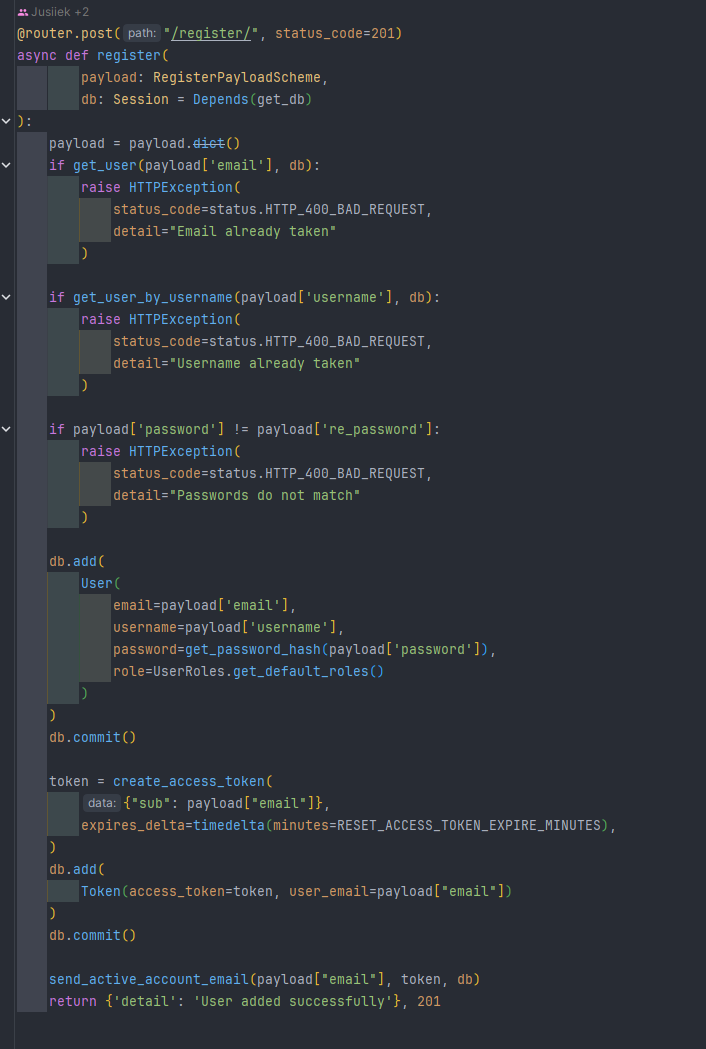
\includegraphics[width=0.7\textwidth]{chapters/chapter_8/screens/rejestracja_backend}
    \caption{Implementacja kodu rejestracji użytkownika w backendzie.}
    \label{img:rejestracja_backend}
\end{figure}

\subsubsection{Aplikacja moblina i aplikacja webowa}
Aby założyć konto, użytkownik musi wypełnić formularz rejestracyjny wymagający podania nazwy użytkownika, adresu email oraz hasła wpisanego jednakowego do dwóch pól w celach jego walidacji. Aplikacja pozwoli na utworzenie konta jedynie jeżeli:

\begin{itemize}
    \item Pseudonim zawiera od 3 do 20 znaków i składa się wyłącznie z liter, cyfr, lub podkreślników
    \item Adres e-mail jest dostarczony w prawidłowym dla niego formacie
    \item Hasło posiada co najmniej 8 znaków
    \item Hasło wpisane oba pola walidacyjne jest w nich takie samo
    \item Adres e-mail i nazwa użytkownika są unikalne (czyli w bazie danych nie są przypisane do żadnego innego konta)
\end{itemize}

Po zatwierdzeniu prawidłowych danych aplikacja informuje komunikatem o udanym utworzeniu konta. Użytkownik zostaje przeniesiony do strony logowania. W przypadku podania nieprawidłowych danych, użytkownik nie zostanie zarejestrowany i zostanie powiadomiony komunikatem w aplikacji o błędzie.

\begin{figure}[H]
    \centering
    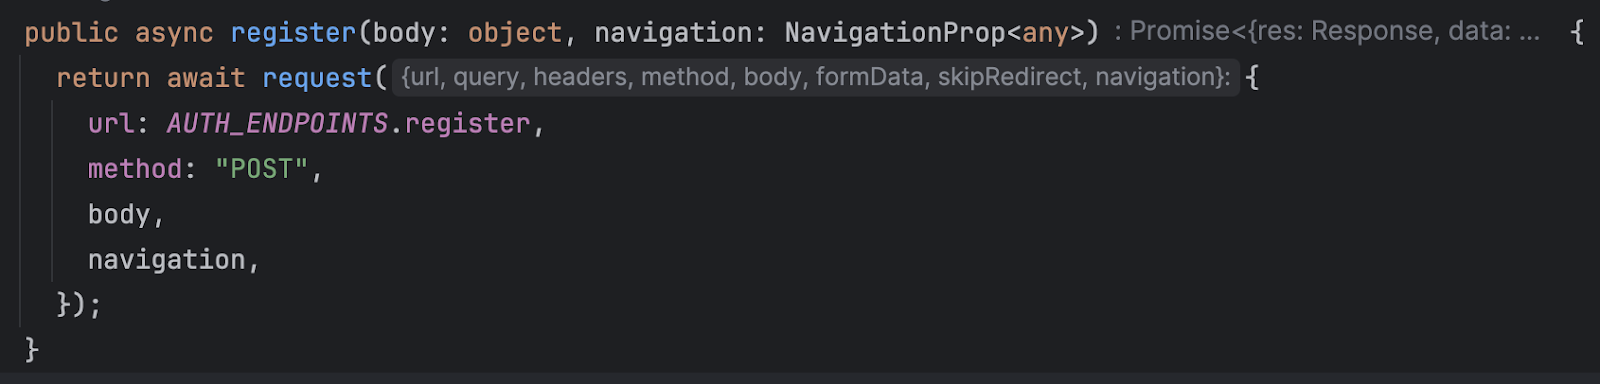
\includegraphics[width=0.7\textwidth]{chapters/chapter_8/screens/rejestracja_mobile}
    \caption{Metoda “register” w serwisie Auth zastosowana w aplikacji mobilnej.}
    \label{img:rejestracja_mobile}
\end{figure}

\begin{figure}[H]
    \centering
    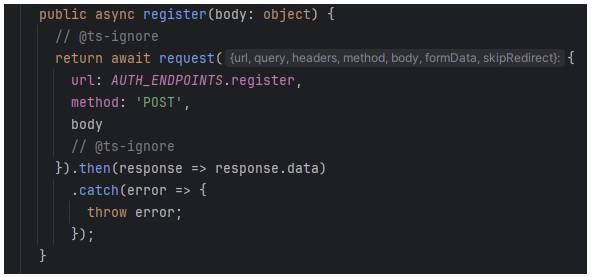
\includegraphics[width=0.7\textwidth]{chapters/chapter_8/screens/rejestracja_web}
    \caption{Metoda “register” w serwisie AuthService zastosowana w aplikacji webowej.}
    \label{img:rejestracja_web}
\end{figure}

Powyższe funkcję wysyłają asynchroniczne żądanie POST do serwera w celu rejestracji nowego użytkownika. Metoda przekazuje dane rejestracyjne w treści żądania, a następnie zwraca czy żądanie zostało obsłużone.

\subsection{Logowanie do systemu}
Funkcjonalność umożliwiająca logowanie do aplikacji

\subsubsection{Backend}
Po wysłaniu requesta na przez aplikację webową lub mobilną api wyciąga przesłane dane, weryfikuje je.
Weryfikacja odbywa się za pomocą funkcji \texttt{authenticate\_user} zaimportowaną z utils’ów.
Ta najpierw próbuje wyciągnąć z użytkownika z bazy, który posiada wysłany e-mail. Potem, jeżeli użytkownik istnieje, sprawdzamy hasło metodą klasową \texttt{verify\_password}. Jeśli wszystko przebiegło pomyślnie, użytkownikowi zostanie zwrócony token autoryzacji i dane użytkownika. W przeciwnym razie zwrócona wiadomość i błędnie wprowadzonych danych.

\begin{figure}[H]
    \centering
    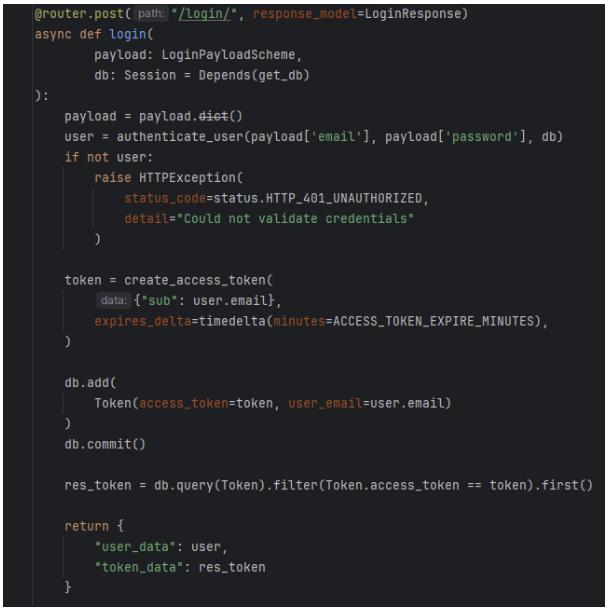
\includegraphics[width=0.7\textwidth]{chapters/chapter_8/screens/logowanie_backend}
    \caption{Implementacja kodu logowania użytkownika w backendzie.}
    \label{img:logowanie_backend}
\end{figure}

\subsubsection{Aplikacja mobilna i aplikacja webowa}
Na stronie logowania, użytkownik musi wypełnić formularz wymagający uzupełnienia pól adres email oraz hasło. Po zatwierdzeniu danych i ich weryfikacji pojawia się komunikat o zalogowaniu użytkownika, a następnie użytkownik zostanie przeniesiony na stronę główną. W przypadku podania nieprawidłowych danych, użytkownik nie zostanie zalogowany i zostanie poinformowany komunikatem o błędzie.

\begin{figure}[H]
    \centering
    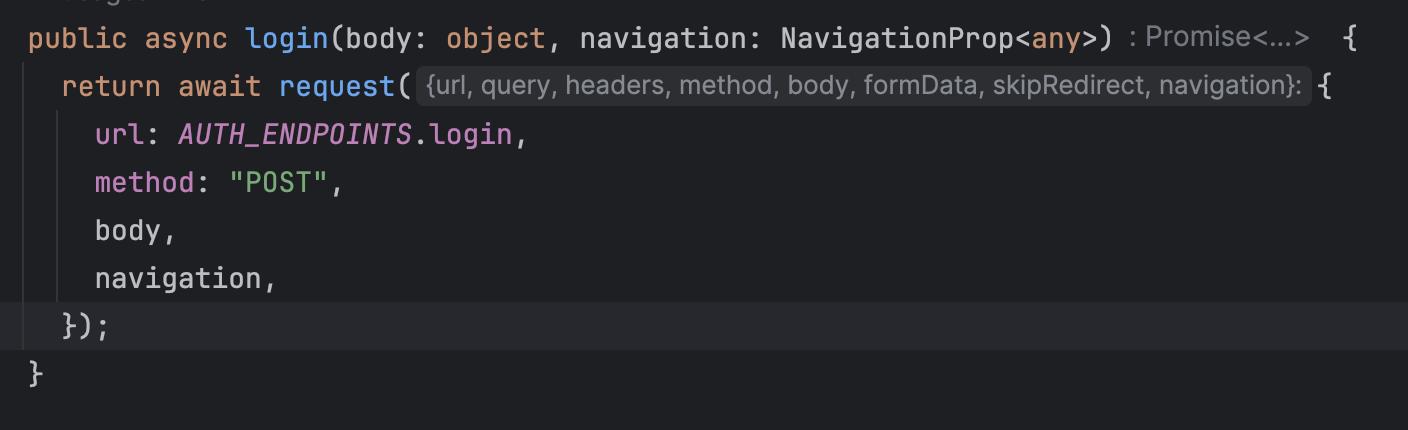
\includegraphics[width=0.7\textwidth]{chapters/chapter_8/screens/logowanie_mobile}
    \caption{Metoda “login” zastosowana w aplikacji mobilnej.}
    \label{img:logowanie_mobile}
\end{figure}

\begin{figure}[H]
    \centering
    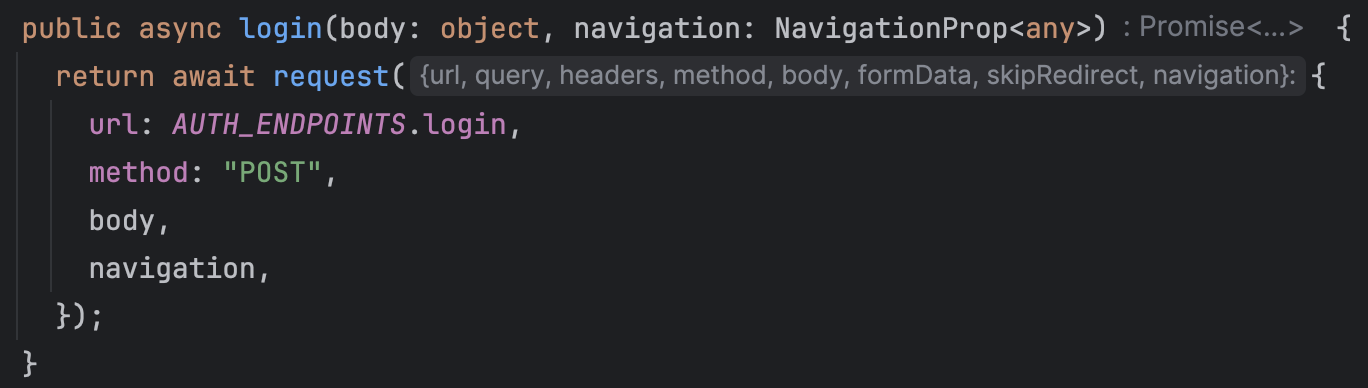
\includegraphics[width=0.7\textwidth]{chapters/chapter_8/screens/logowanie_web}
    \caption{Metoda “login” zastosowana w aplikacji webowej.}
    \label{img:logowanie_web}
\end{figure}

Użyta w powyższych metodach funkcja \texttt{ActiveUser.set(data)} zapisuje dane zalogowanego użytkownika w lokalnym stanie aplikacji. Dzięki temu, informacje o użytkowniku, takie jak token autoryzacyjny, mogą być łatwo dostępne w całej aplikacji. Pozwala to na:

\begin{itemize}
    \item Personalizację interfejsu użytkownika (np. wyświetlanie nazwy użytkownika)
    \item Umożliwienie dostępu do zasobów, które wymagają uwierzytelnienia
    \item Przechowywanie sesji użytkownika, aby mógł pozostać zalogowany pomiędzy różnymi wizytami na stronie
\end{itemize}

\subsection{Wylogowanie z systemu}
Funkcjonalność pozwalająca na wylogowanie użytkownika.

\subsubsection{Backend}
Po kliknięciu wyloguj w aplikacji mobilnej czy w webowej, zostaje wysłany request na api, który dodaje aktualnie używany token do listy nieaktualnych tokenów.

\begin{figure}[H]
    \centering
    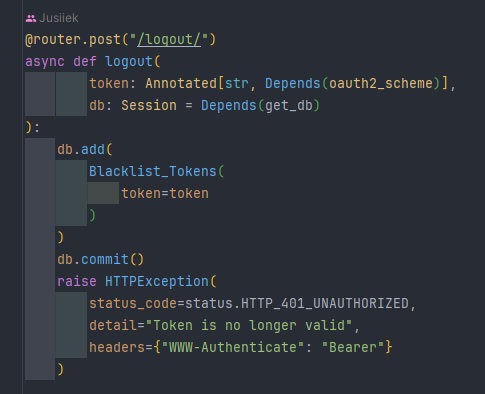
\includegraphics[width=0.7\textwidth]{chapters/chapter_8/screens/wylogowanie_backend}
    \caption{Implementacja kodu wylogowania użytkownika w backendzie.}
    \label{img:wylogowanie_backend}
\end{figure}

\subsubsection{Aplikacja mobilna i aplikacja webowa}
Aby wylogować się z aplikacji, użytkownik musi kliknąć w nawigacji logout. Po kliknięciu przycisku, dane użytkownika zostaną usunięte z pamięci lokalnej. Token autoryzacyjny użytkownika utworzony przy logowaniu zostanie dodany w bazie danych do tabeli zawierającej nieaktywne tokeny.

\begin{figure}[H]
    \centering
    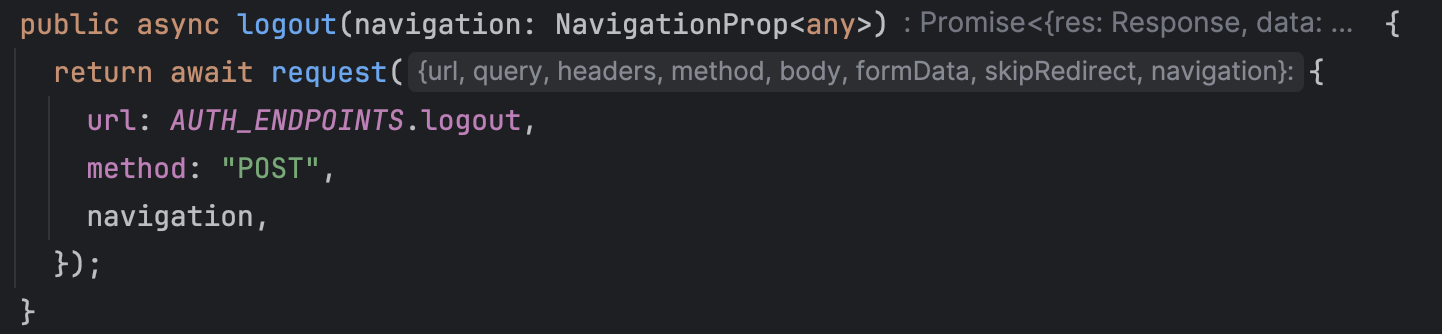
\includegraphics[width=0.7\textwidth]{chapters/chapter_8/screens/wylogowanie_mobile}
    \caption{Metoda “logout” zastosowana w aplikacji mobilnej.}
    \label{img:wylogowanie_mobile}
\end{figure}

\begin{figure}[H]
    \centering
    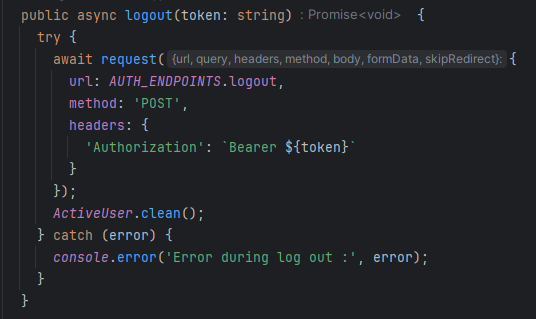
\includegraphics[width=0.7\textwidth]{chapters/chapter_8/screens/wylogowanie_web}
    \caption{Metoda “logout” zastosowana w aplikacji webowej.}
    \label{img:wylogowanie_web}
\end{figure}

Powyższe fragmenty serwisu odpowiadają za usunięcie danych użytkownika z pamięci lokalnej wykorzystujący endpoint dezaktywujący token autoryzacji.

\subsection{Edycja danych użytkownika}
Funkcjonalność umożliwiająca  edycję danych użytkownika.

\subsubsection{Backend}
Aplikacje frontendowe wysyłają dane do aktualizacji np. email. Jedynym obowiązkowym atrybutem przy aktualizacji jest \texttt{current\_password}. Po zweryfikowaniu zgodności hasła, system przystępuje do zmiany danych wprowadzonych przez użytkownika. Na koniec zostają zwrócone użytkownika z poprawionym polami.

\begin{figure}[H]
    \centering
    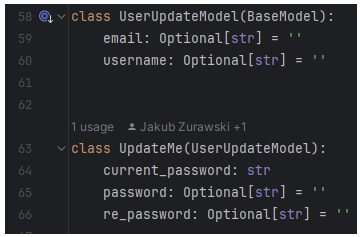
\includegraphics[width=0.5\textwidth]{chapters/chapter_8/screens/edit_user_backend_1}
    \caption{Implementacja klas modeli "UserUpdateModel" i "UpdateMe" w backendzie.}
    \label{img:edit_user_backend_1}
\end{figure}

\begin{figure}[H]
    \centering
    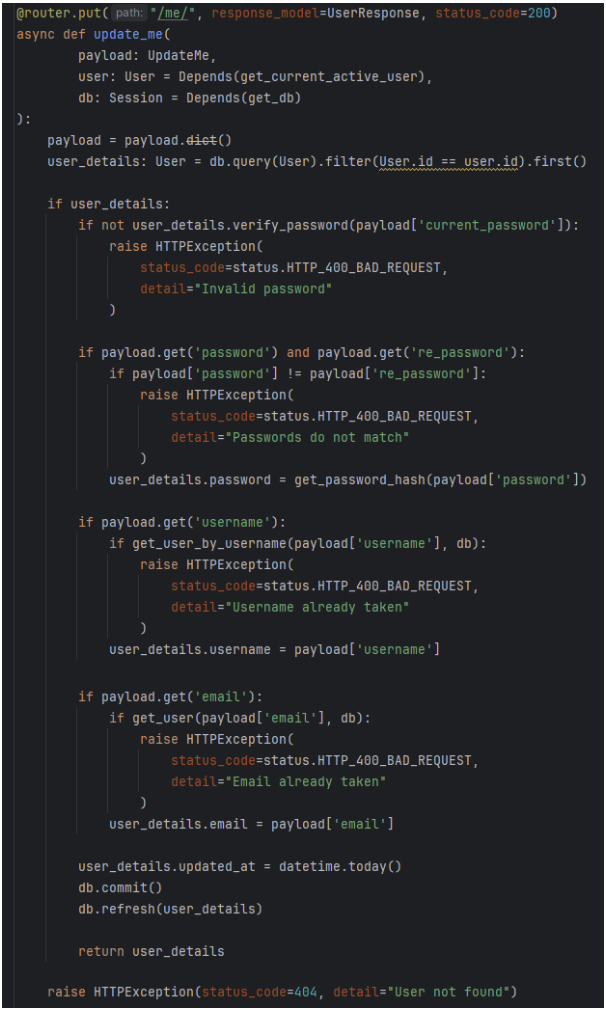
\includegraphics[width=0.7\textwidth]{chapters/chapter_8/screens/edit_user_backend_2}
    \caption{Implementacja kodu zmiany danych użytkownika w backendzie.}
    \label{img:edit_user_backend_2}
\end{figure}

\subsubsection{Aplikacja mobilna i aplikacja webowa}
W celu zmiany danych użytkownika, takich jak avatar, nickname, adres email czy hasło, użytkownik może skorzystać z odpowiednich formularzy dostępnych na stronie profilu użytkownika. Każda zmiana (za wyjątkiem zmiany avatara) wymaga uwierzytelnienia przez podanie aktualnego hasła. Poniżej opisane są poszczególne procesy.

\begin{figure}[H]
    \centering
    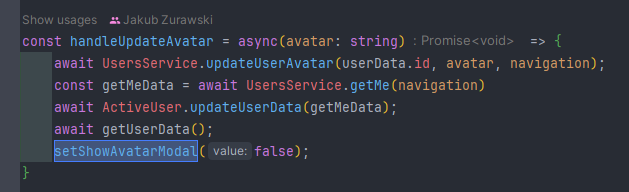
\includegraphics[width=0.7\textwidth]{chapters/chapter_8/screens/edit_user_mobile}
    \caption{Funkcja “handleAvatarSelect” zastosowany w aplikacji mobilnej.}
    \label{img:edit_user_mobile}
\end{figure}

\begin{figure}[H]
    \centering
    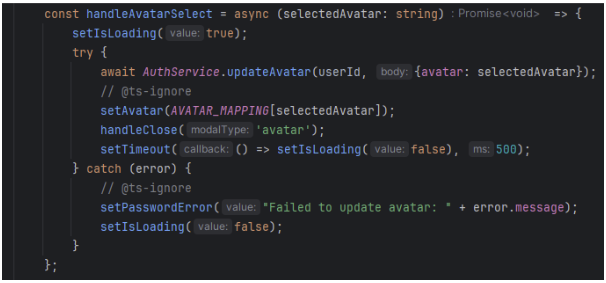
\includegraphics[width=0.7\textwidth]{chapters/chapter_8/screens/edit_user_web}
    \caption{Funkcja “handleAvatarSelect” zastosowany w aplikacji webowej.}
    \label{img:edit_user_web}
\end{figure}

\textbf{Zmiana avatara}\\
Aby zmienić avatar, użytkownik musi wybrać nowy avatar z dostępnych opcji. Po dokonaniu wyboru aplikacja wysyła żądanie do serwera w celu aktualizacji avatara. Po pomyślnej aktualizacji użytkownik zobaczy nowy avatar na stronie profilu oraz w widoku statystyk.\\


\textbf{Zmiana pseudonimu}\\
Aby zmienić pseudonim, użytkownik musi wprowadzić nowy pseudonim oraz aktualne hasło w odpowiednim formularzu. Po zatwierdzeniu formularza dane są walidowane:
\begin{itemize}
    \item Pseudonim musi zawierać 3-20 znaków i składać się wyłącznie z liter, cyfr lub podkreślników
    \item Aktualne hasło musi być poprawne
\end{itemize}
Jeśli dane są poprawne, aplikacja wysyła żądanie do serwera w celu aktualizacji pseudonimu. Po pomyślnej aktualizacji nowy pseudonim będzie wyświetlany na stronie profilu.\\


\textbf{Zmiana adresu email}\\
Aby zmienić adres email, użytkownik musi wprowadzić nowy adres email oraz aktualne hasło w odpowiednim formularzu. Po zatwierdzeniu formularza dane są walidowane:
\begin{itemize}
    \item Adres email musi mieć poprawny format
    \item Aktualne hasło musi być poprawne
\end{itemize}
Jeśli dane są poprawne, aplikacja wysyła żądanie do serwera w celu aktualizacji adresu email. Po pomyślnej aktualizacji użytkownik będzie logował się nowym adresem email.\\


\textbf{Zmiana hasła}\\
Aby zmienić hasło, użytkownik musi wprowadzić aktualne hasło, nowe hasło oraz potwierdzenie nowego hasła w odpowiednim formularzu. Po zatwierdzeniu formularza dane są walidowane:
\begin{itemize}
    \item Nowe hasło musi mieć co najmniej 8 znaków
    \item Potwierdzenie nowego hasła musi być zgodne z nowym hasłem
    \item Aktualne hasło musi być poprawne
\end{itemize}
Jeśli dane są poprawne, aplikacja wysyła żądanie do serwera w celu aktualizacji hasła.

\subsection{Usunięcie konta użytkownika}
Funkcjonalność umożliwiająca usunięcie konta użytkownika.

\subsubsection{Backend}
Aplikacje frontendowe wysyłają na api email użytkownika i hasło. Api sprawdza poprawność danych, następnie usuwa konto użytkownika.

\begin{figure}[H]
    \centering
    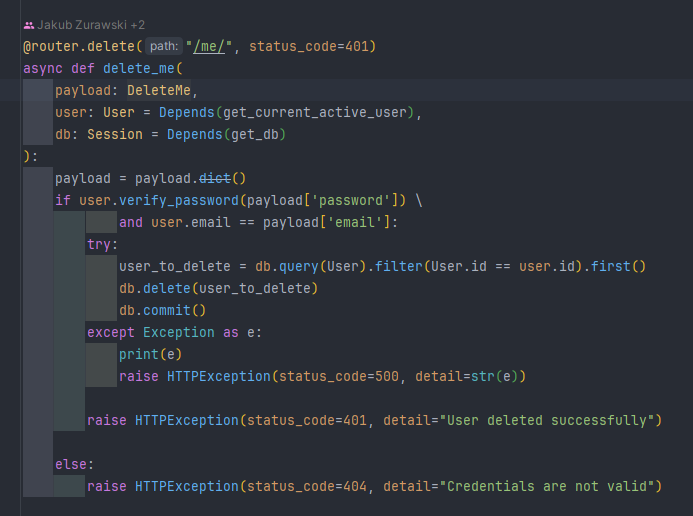
\includegraphics[width=0.7\textwidth]{chapters/chapter_8/screens/delete_user_backend}
    \caption{Implementacja kodu usunięcia użytkownika w backendzie.}
    \label{img:delete_user_backend}
\end{figure}

\subsubsection{Aplikacja moblina}
Użytkownik jest proszony o potwierdzenie czy aby na pewno chce usunąć konto. Po zatwierdzeniu zostaje przekierowany do formularza gdzie podaje email oraz hasło, które po zatwierdzeniu zostają wysłane na api.

\begin{figure}[H]
    \centering
    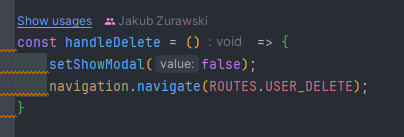
\includegraphics[width=0.7\textwidth]{chapters/chapter_8/screens/delete_user_mobile_1}
    \caption{Wywołanie funkcji “handleDelete” zastosowanego w aplikacji mobilnej.}
    \label{img:delete_user_mobile_1}
\end{figure}

\begin{figure}[H]
    \centering
    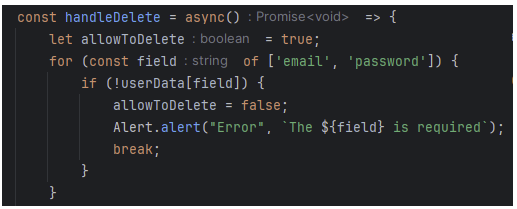
\includegraphics[width=0.7\textwidth]{chapters/chapter_8/screens/delete_user_mobile_2}
    \caption{Funkcja “handleDelete” zastosowany w aplikacji mobilnej.}
    \label{img:delete_user_mobile_2}
\end{figure}

\subsubsection{Aplikacja webowa}

Jeżeli po potwierdzeniu wyboru prawidłowym hasłem, funkcja wykryje error 401 (Unauthorized), oznaczać to będzie że konto zostało usunięte. Następnie pojawia się komunikat o usunięciu który przekierowuje do strony logowania

\begin{figure}[H]
    \centering
    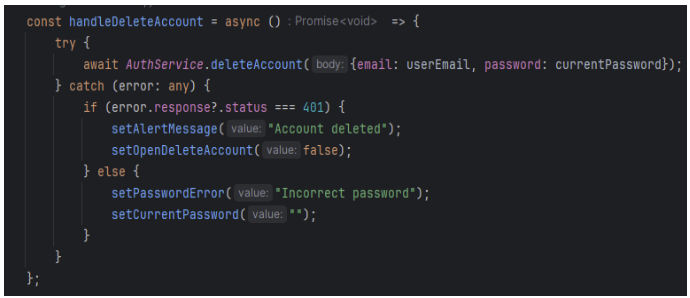
\includegraphics[width=0.7\textwidth]{chapters/chapter_8/screens/delete_user_web}
    \caption{Funkcja “handleDelete” zastosowany w aplikacji webowej.}
    \label{img:delete_user_web}
\end{figure}

\subsection{Tworzenie talii fiszek}

Funkcjonalność umożliwiająca tworzenie talii fiszek.

\subsubsection{Backend}

Utworzono metodę post, która umożliwia tworzenie talii o podanej nazwie i kategorii. Do tworzenia fiszki używana jest osobna metoda post, która przyjmuje treść dla przedniej i tylnej strony karty, a także id talii do, której utworzona fiszka zostanie przypisana.

\begin{figure}[H]
    \centering
    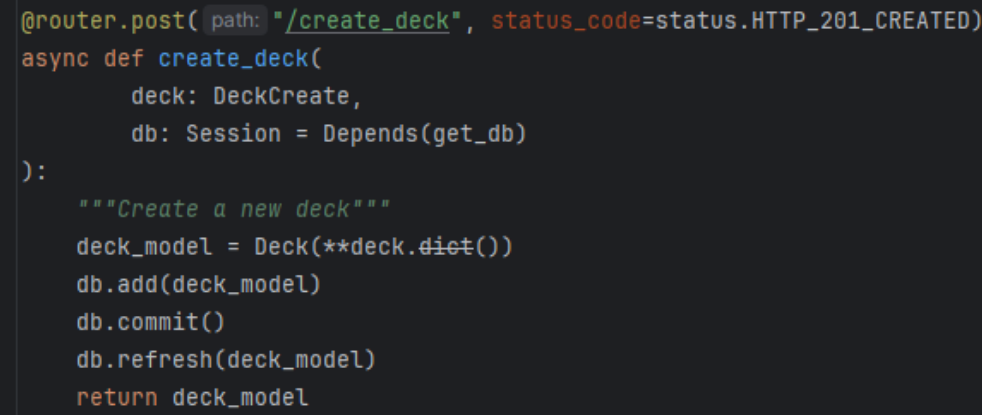
\includegraphics[width=0.7\textwidth]{chapters/chapter_8/screens/create_deck_backend}
    \caption{Logika tworzenia decku po stronie serwera.}
    \label{img:create_deck_backend}
\end{figure}

\begin{figure}[H]
    \centering
    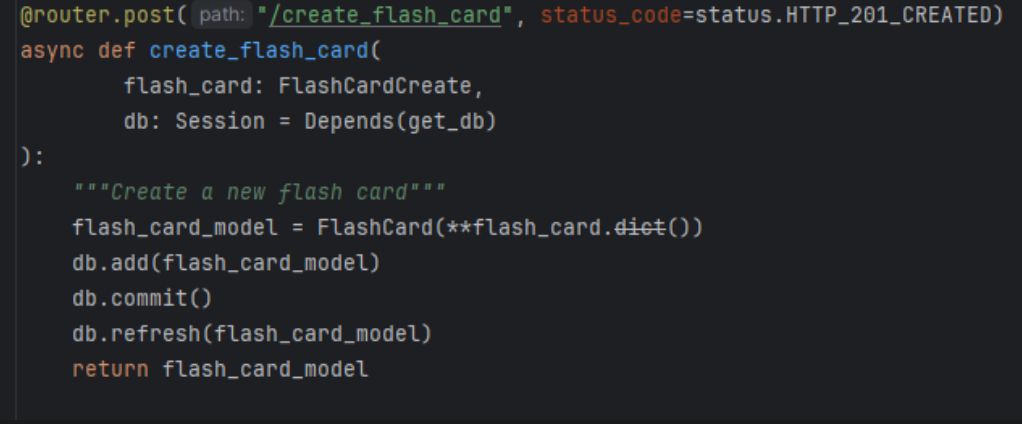
\includegraphics[width=0.7\textwidth]{chapters/chapter_8/screens/create_flash_card_backend}
    \caption{Logika tworzenia fiszek po stronie serwera.}
    \label{img:create_flash_card_backend}
\end{figure}

\subsubsection{Aplikacja mobilna}
Dodanie fiszki jest możliwe po przejściu do widoku jej tworzenia z podglądu wybranej talii. Wymagane jest uzupełnienie pól przedniej i tylnej strony fiszki. Tworzenie odbywa się przez wysłanie danych do odpowiedniego endpointu.

\begin{figure}[H]
    \centering
    \includegraphics[width=0.7\textwidth]{chapters/chapter_8/screens/create_deck_mobile}
    \caption{Funkcja obsługująca tworzenie nowej fiszki..}
    \label{img:create_deck_mobile}
\end{figure}

\subsubsection{Aplikacja webowa}

Użytkownik aby utworzyć talię musi wypełnić pole tekstowe dla nazwy i kategorii talii, następnie musi uzupełnić treść dla przedniej i tylnej strony fiszki. Po kliknięciu create deck dane z formularzy zostają przekazane do funkcji, która zebrane dane przekazuje do serwisu odpowiedzialnego za komunikację z endpointem do tworzenia talii i endpointem do tworzenia fiszki.

\begin{figure}[H]
    \centering
    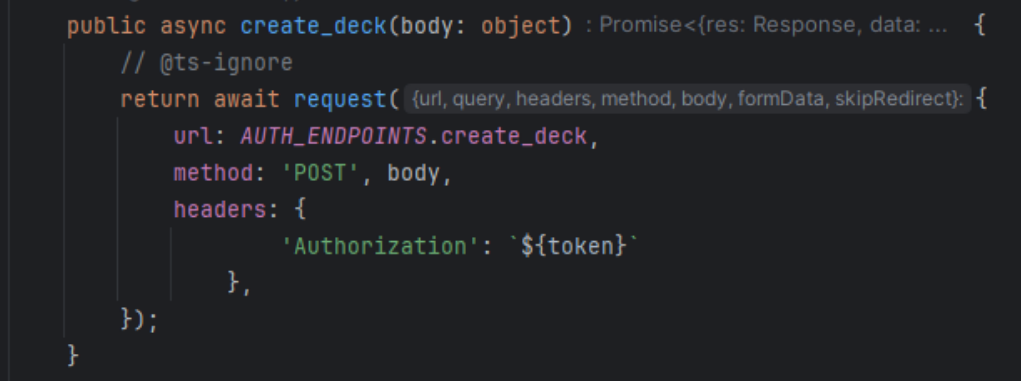
\includegraphics[width=0.7\textwidth]{chapters/chapter_8/screens/create_deck_web}
    \caption{Funkcja serwisu odpowiedzialna za komunikację z endpointem do tworzenia decku.}
    \label{img:create_deck_web}
\end{figure}

\begin{figure}[H]
    \centering
    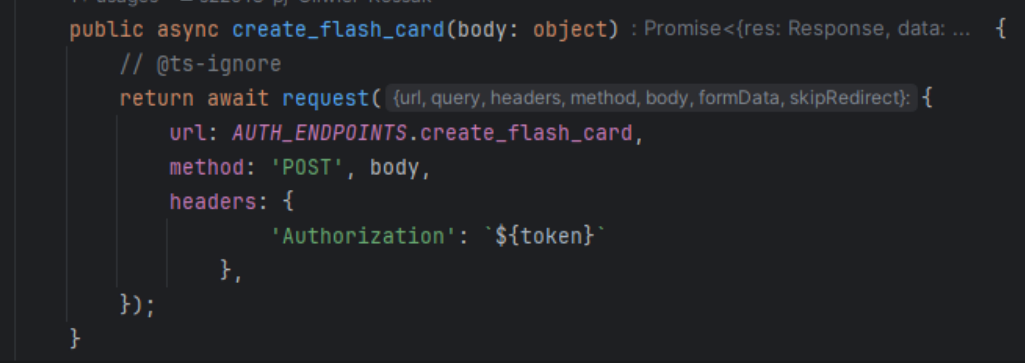
\includegraphics[width=0.7\textwidth]{chapters/chapter_8/screens/create_flash_card_web}
    \caption{Funkcja serwisu odpowiedzialna za komunikację z endpointem do tworzenia fiszki.}
    \label{img:create_flash_card_web}
\end{figure}

\subsection{Usunięcie talii fiszek}

Funkcjonalność umożliwiająca usunięcie talii fiszek.

\subsubsection{Backend}

Został utworzony endpoint delete_deck, która pozwala na usunięcie talii o podanym id wraz z wszystkimi powiązanymi fiszkami.

\begin{figure}[H]
    \centering
    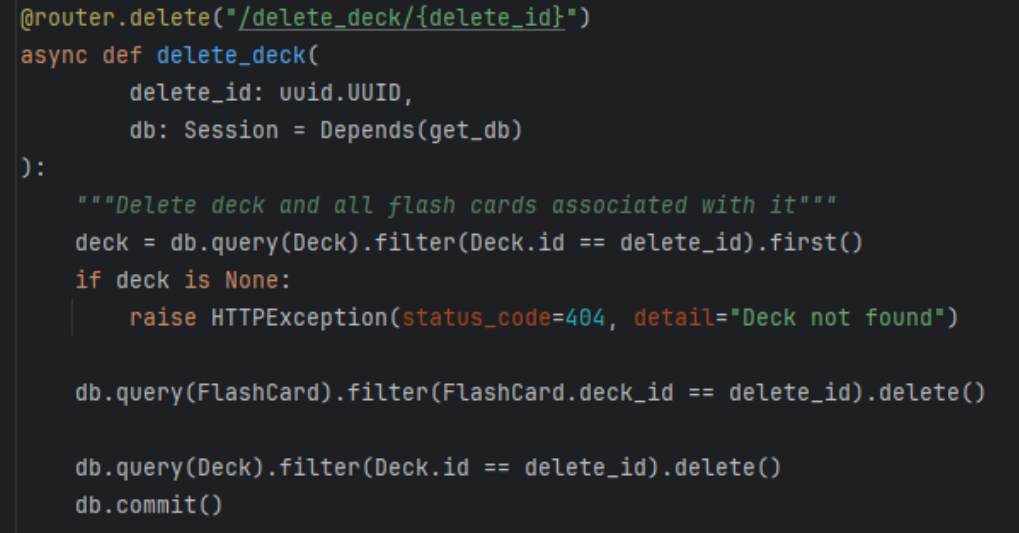
\includegraphics[width=0.7\textwidth]{chapters/chapter_8/screens/delete_deck_backend}
    \caption{Logika usuwająca talie i wszystkie należące do niej fiszki.}
    \label{img:delete_deck_backend}
\end{figure}


\subsubsection{Aplikacja moblina}
Usunięcie talii jest możliwe z poziomu jej opcji. Po wybraniu tej opcji do api zostaje wysłane zapytanie o usunięcie talii. W zapytaniu przekazywane jest id decku.

\begin{figure}[H]
    \centering
    \includegraphics[width=0.7\textwidth]{chapters/chapter_8/screens/delete_deck_mobile}
    \caption{Funkcja odpowiedzialna za obsługę usunięcia decku.}
    \label{img:delete_deck_mobile}
\end{figure}

\subsubsection{Aplikacja webowa}

Użytkownik aby usunąć talię klika w opcje, następnie wybiera delete deck. Po kliknięciu id aktualnej talii zostaje pobrane z pamięci lokalnej i przekazane do serwisu, który łączy się z bakcendowym endpoint em do usuwania talii. Endpoint usuwa z bazy danych talię o podanym id i wszystkie należące do niego fiszki.

\begin{figure}[H]
    \centering
    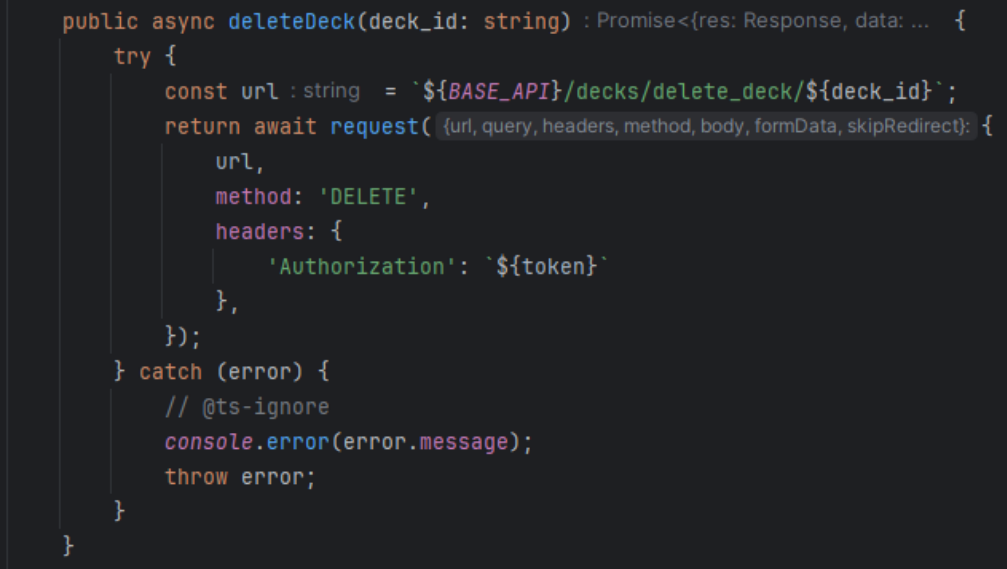
\includegraphics[width=0.7\textwidth]{chapters/chapter_8/screens/delete_deck_web}
    \caption{Funkcja serwisu odpowiedzialna za komunikację z endpointem do usuwania decku.}
    \label{img:delete_deck_web}
\end{figure}














